\chapter{Test Implementation}
\label{cap:real_implementation}

To validate the proposed architecture and demonstrate its practical application, a real-world problem was selected for a proof of concept (PoC) implementation. Testing the architecture in a real-world scenario ensures that the system can meet the demands and challenges faced by actual users. In this PoC, however, actual users were simulated using MQTT clients to replicate the data upload patterns and volume expected in a real-world deployment. This approach highlights the scalability, reliability, and cloud-agnostic capabilities of the architecture when handling diverse workloads, making it an essential step for proving the viability of the solution.

The selected real-world problem comes from a company specializing in high-performance protective gear and technical apparel for motorsports and action sports. This case study aimed to develop a system that could analyze data from Inertial Measurement Units (IMUs) embedded in riders’ suits, providing feedback on performance, safety metrics, and crash detection. The client intends to use this system for both private users and professional motorsport pilots to improve riding performance and ensure safety.

Given the sporadic and intensive data generated by different types of users, the system needed to handle diverse upload patterns, manage a large volume of data, and provide insights in critical cases (such as detecting a crash). Testing the architecture in this context provides crucial feedback on the system’s ability to scale, manage data efficiently, and provide data analysis across different cloud platforms, such as Aruba Cloud and Azure.

\section{Why testing the architecture on a real-world problem?}
\label{sec:real_world_problem}

Implementing the architecture in a real-world scenario provides several benefits beyond theoretical testing:
\begin{itemize}
    \item \textbf{Scalability Testing}: Since users upload varying amounts of data based on actual usage patterns, this helps validate the system’s ability to scale both horizontally and vertically.
    \item \textbf{Performance and Resource Utilization}: The architecture’s ability to manage the load under real conditions, such as spikes in data uploads, can be accurately measured, enabling optimization of resource utilization.
    \item \textbf{Cloud-Agnostic Validation}: Testing across multiple cloud providers (in this case, Aruba Cloud and Azure) proves that the architecture can operate without significant modification, reducing vendor lock-in.
    \item \textbf{User Interaction and Feedback}: Real-world testing provides insights into how users would interact with the system, enabling further refinement of the user experience and data handling mechanisms.
\end{itemize}

By addressing these aspects, the PoC implementation of the system offers a comprehensive assessment of the architecture’s practical performance and highlights potential areas for improvement, ensuring that it can support future real-world deployments.

\section{Implementation of the data collection layer}
\label{sec:implementation_data_collection}

The data collection layer is responsible for gathering data from the biker suits and uploading it to cloud storage for further processing. This layer handles two key tasks: MQTT data ingestion from the IMUs and uploading archived data.

\subsection{Data ingestion from MQTT}
To handle MQTT data ingestion, the system uses an MQTT broker, specifically the EMQX broker, which was selected for its scalability and cloud-agnostic nature. The MQTT broker receives data from the IMUs in JSON format, which is published to specific MQTT topics based on the type of data and the user.

In the PoC, the IMUs were simulated using the MQTTX tool to emulate data from the biker suits. Each device published JSON messages containing timestamps and sensor data (such as acceleration and gyroscope readings). The MQTT broker was configured on both Aruba Cloud and Azure servers to validate the cloud-agnostic nature of the architecture.

\textbf{Implementation Details}:
\begin{itemize}
    \item \textbf{MQTT Topics}: Each biker suit publishes data to its own MQTT topic, allowing easy organization and routing of messages.
    \item \textbf{Broker Testing}: The broker was tested by simulating data uploads using MQTTX clients. The system successfully received the data, confirming the stability and scalability of the MQTT broker.
\end{itemize}

\subsubsection{Preprocessing pipeline}
After receiving data from the MQTT broker, the next step in the data collection layer is the preprocessing pipeline, which converts the incoming JSON data into a CSV format for easier processing and storage. The pipeline was implemented using a Python script that subscribes to the MQTT broker, parses the JSON data, and stores it locally. The code of the script is provided in Section \ref{sec:prprocessing_impl}. Sucessively, another script uploads the data to the object storage, and its code is provided in Section \ref{sec:upload_cloudcloud_impl}.

\textbf{Implementation Details}:
\begin{itemize}
    \item \textbf{Data Parsing}: The pipeline extracts timestamps and sensor values from the JSON messages, converts them into CSV rows, and stores them in object storage.
    \item \textbf{Cloud-Agnostic Storage}: The CSV files were uploaded to object storage on both Azure Blob Storage and Aruba Cloud, proving that the preprocessing pipeline works across different cloud platforms.
\end{itemize}

\subsection{Data ingestion from archived data}
\label{sec:archived_data_ingestion}

In addition to the MQTT-based data ingestion from IoT devices, the system must also support the ingestion of archived data, typically collected and stored locally. This archived data needs to be uploaded to cloud storage for further processing and analysis. The ingestion of archived data ensures that both historical and MQTT-ingested data can be integrated into the system seamlessly, providing a comprehensive view of the dataset for users and allowing retrospective analyses.

In this implementation, archived data is expected to be stored locally in CSV format. A Python script is used to upload this archived data from an on-premise location to the cloud object storage, where it can be accessed by the data analysis pipeline. The script handles large batch uploads and is designed to operate across different cloud environments (such as Azure Blob Storage and Aruba Cloud Object Storage), maintaining the cloud-agnostic nature of the system. The code for the implementation is provided in Section \ref{sec:upload_cloudcloud_impl}.

\textbf{Implementation Details}:
\begin{itemize}
    \item \textbf{File Structure}: The archived data is expected to follow a structured format (e.g., CSV) that is compatible with the analysis pipelines.
    \item \textbf{Upload Mechanism}: The script leverages the cloud provider's API to handle file uploads, ensuring compatibility with various storage providers.
    \item \textbf{Batch Processing}: The system supports bulk uploads of multiple files, making it efficient for handling large datasets. The script can upload entire directories or specific files as needed.
    \item \textbf{Storage Confirmation}: After each file is uploaded, the system verifies its successful transfer to the cloud storage and logs any failures for troubleshooting.
\end{itemize}

\section{Implementation of the data storage layer}
\label{sec:implementation_data_storage}

The data storage layer handles the storage of both raw and processed data in cloud object storage. Object storage was chosen for its scalability and flexibility, allowing the system to manage large volumes of unstructured data efficiently.

\subsection{Object storage configuration}
In the PoC, object storage was set up on both Azure and Aruba Cloud. Separate storage buckets were created to manage raw data, processed analytics, and crash-specific data. The separation of data ensures that raw sensor data can be archived, while processed data is readily accessible for further analysis or user requests. An example of data stored on Aruba Object Storage and Azure Blob Storage can be seen respectively in Figure \ref{fig:aruba_obj_storage} and \ref{fig:azure_obj_storage}.

\textbf{Implementation Details}:
\begin{itemize}
    \item \textbf{Raw Data Storage}: Data from the biker suits was uploaded to raw data buckets in both Azure and Aruba Cloud Object Storage.
    \item \textbf{Processed Data Storage}: The data analysis component stores results in separate analytics buckets, while crash-specific data is stored in dedicated buckets.
    \item \textbf{Testing}: The storage layer was tested by uploading and retrieving both raw and processed data from the cloud storage services, demonstrating the cloud-agnostic nature of the system.
\end{itemize}

\begin{figure}[htbp]
    \centering
    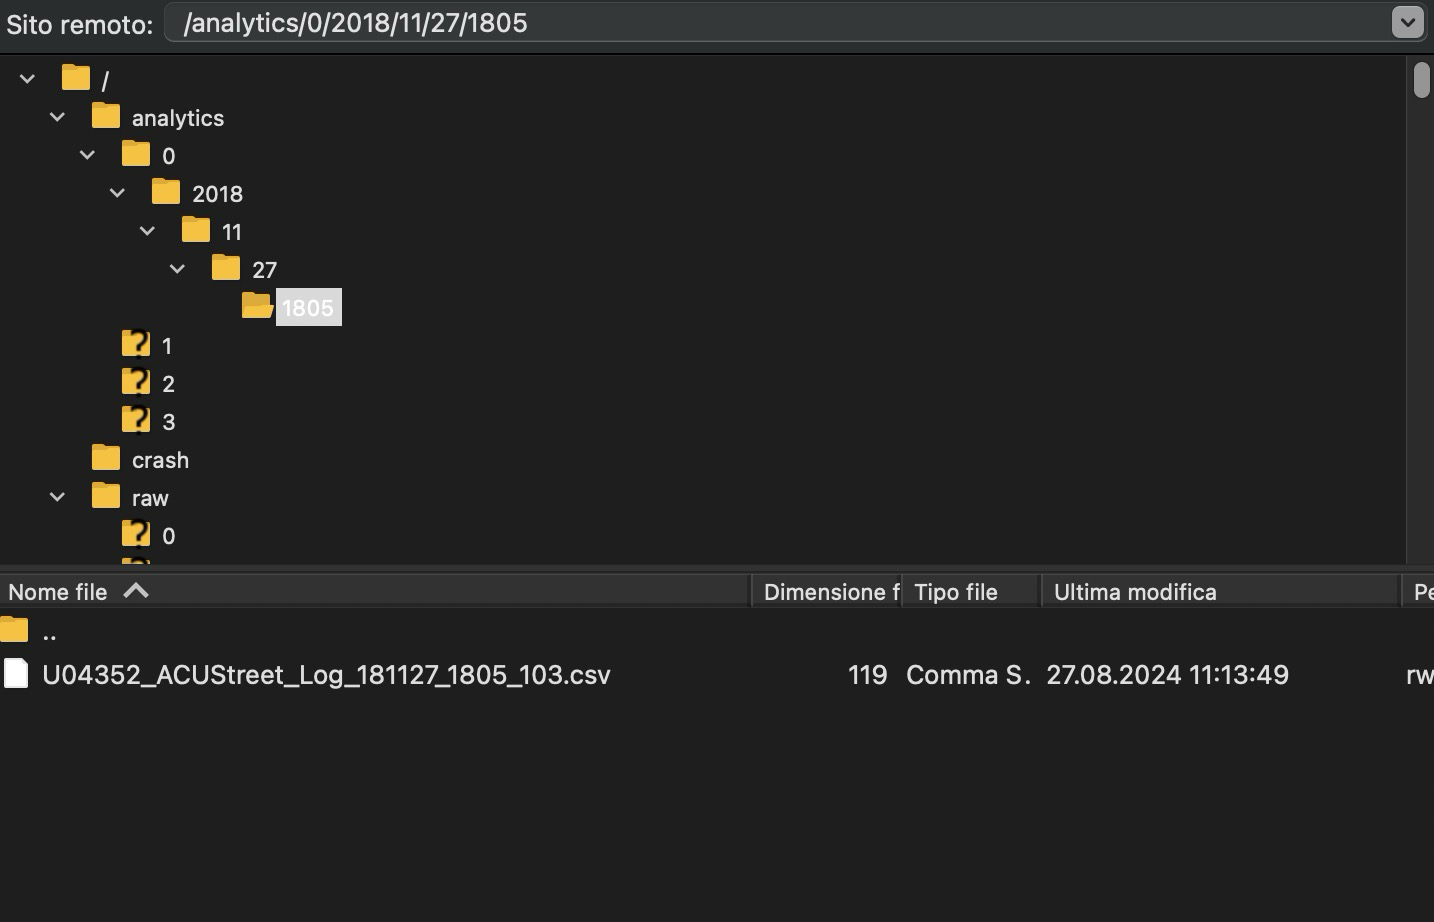
\includegraphics[width=1\textwidth]{Immagini/data_storage.png}
    \caption{Example of data stored on Aruba Object Storage}
    \label{fig:aruba_obj_storage}
\end{figure}

\begin{figure}[htbp]
    \centering
    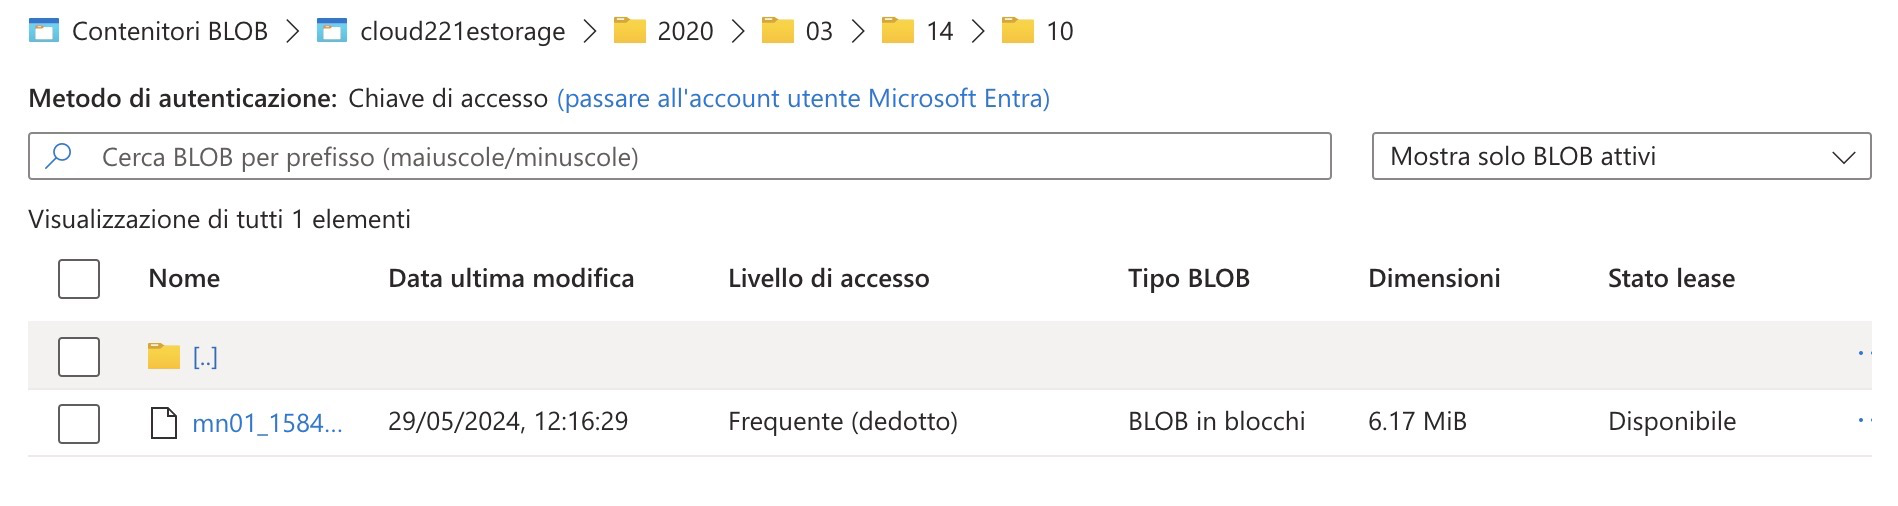
\includegraphics[width=1\textwidth]{Immagini/azure_storage.png}
    \caption{Example of data stored on Azure Blob Storage}
    \label{fig:azure_obj_storage}
\end{figure}


\section{Implementation of the data analysis layer}
\label{sec:implementation_data_analysis}

The data analysis layer is responsible for processing the collected data, running analytics, and storing the results. In this implementation, the data analysis layer retrieves preprocessed data, performs the required analysis, and stores the results back in object storage.

\subsection{Data processing pipeline}
\label{sec:data_processing_pipeline}

The data processing pipeline was implemented using Java. The pipeline reads and processes the preprocessed CSV data stored in object storage. The pipeline performs essential tasks such as calculating average speed, detecting left and right turns, identifying maximum acceleration and deceleration, and flagging potential crash events based on sensor data.

\textbf{Implementation Details}:
\begin{itemize}
    \item \textbf{CSV Data Processing}: The Java function reads the sensor data from a CSV file, processes key metrics such as speed, acceleration, and orientation, and calculates values like the highest acceleration, deceleration, and average speed.
    \item \textbf{Turn Detection}: Left and right turns are detected based on changes in the orientation angle of the rider, derived from chest orientation sensor data. 
    \item \textbf{Storage of Results}: After processing, the calculated metrics are stored in a structured format (e.g., a map) for later storage or further analysis.
\end{itemize}

The processing pipeline reads the CSV data using Apache Commons CSV, a library that simplifies reading and parsing CSV files. The script processes each record, extracting relevant sensor data, performing calculations, and storing the resulting metrics in a key-value format for further use. The following metrics are calculated: highest acceleration, highest deceleration, average speed, and the number of left and right turns.

For more details on the implementation of the data processing function, refer to the code in Section \ref{sec:analysis_fun}, while an example of the result of the analysis process can be seen in figure \ref{fig:analysis}.
\begin{figure}[htbp]
    \centering
    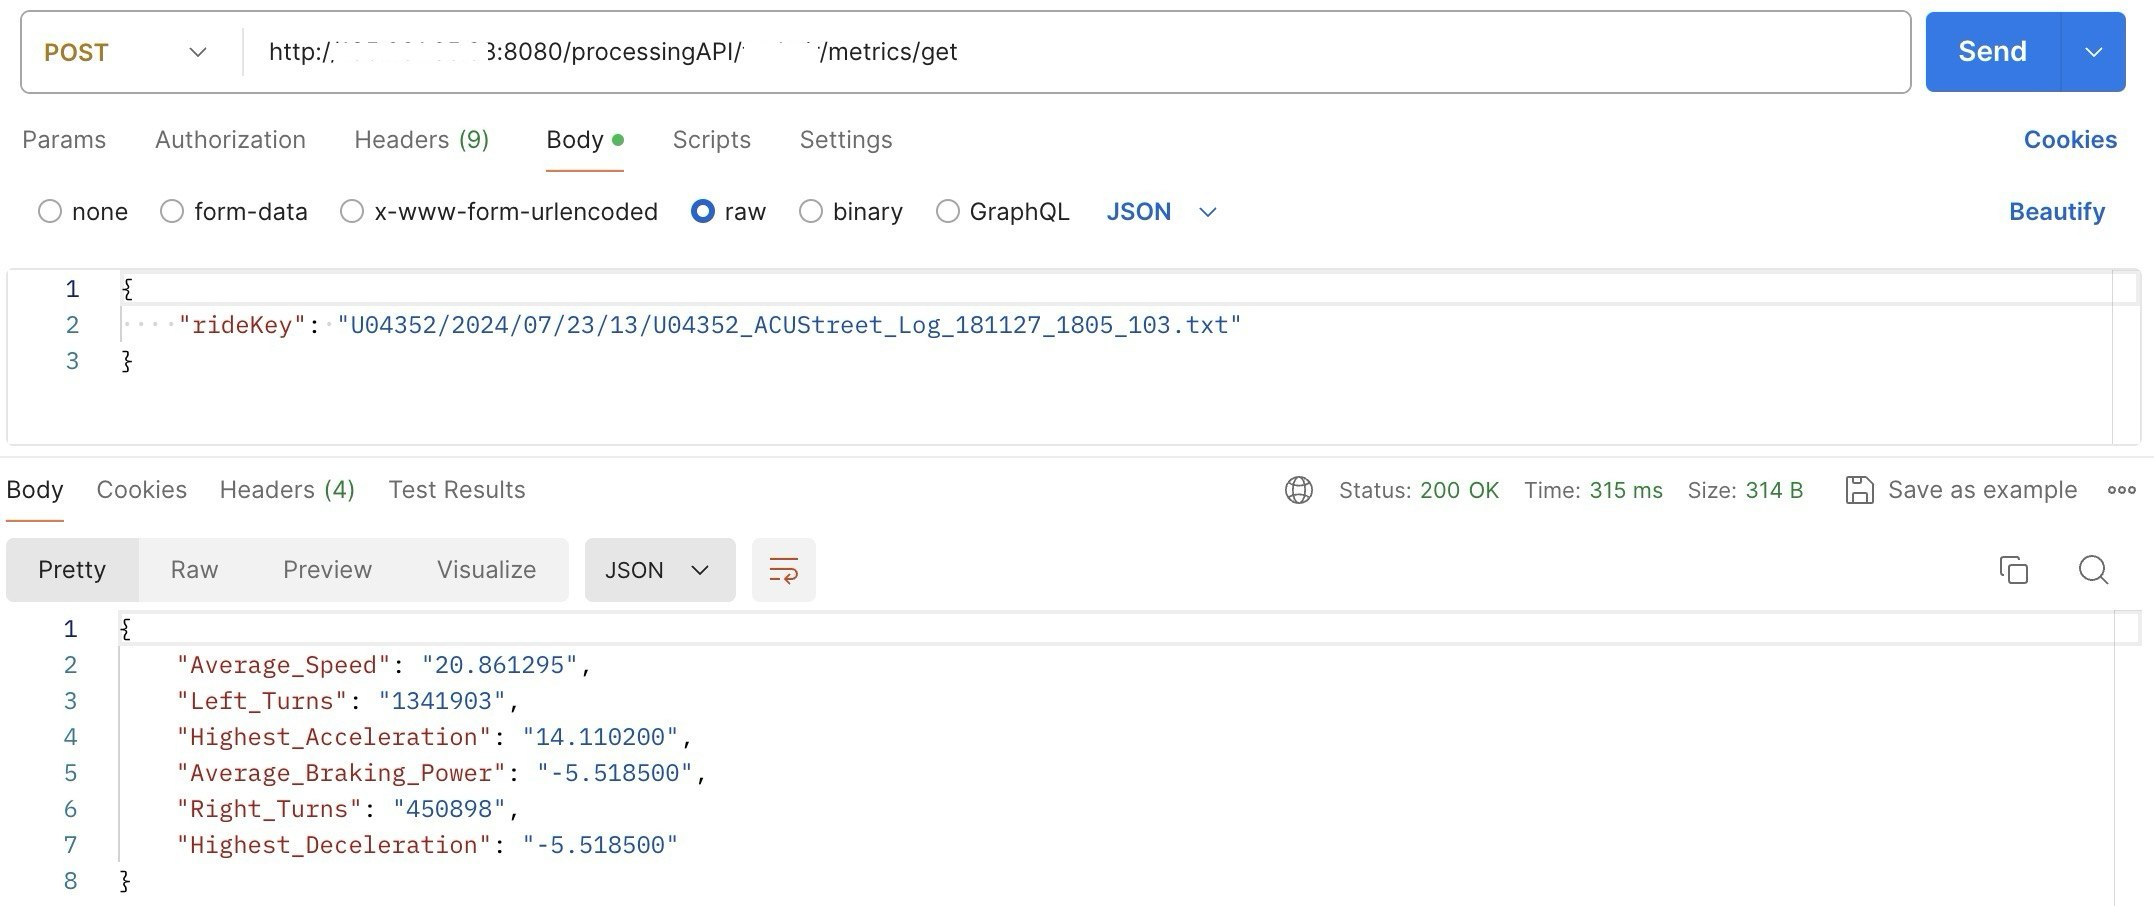
\includegraphics[width=1\textwidth]{Immagini/get_metrics.png}
    \caption{Example of results of the analysis process}
    \label{fig:analysis}
\end{figure}
